\documentclass{article}

\usepackage[utf8]{inputenc}
\usepackage{graphicx} %package to manage images
\usepackage{amsmath}

\usepackage{listings}
\usepackage{placeins}
\usepackage{subcaption}


\usepackage[rightcaption]{sidecap}
\usepackage{wrapfig}
\usepackage{color}

\definecolor{mygreen}{rgb}{0,0.6,0}
\definecolor{mygray}{rgb}{0.5,0.5,0.5}
\definecolor{mymauve}{rgb}{0.58,0,0.82}

\lstset{ %
  backgroundcolor=\color{white},   % choose the background color; you must add \usepackage{color} or \usepackage{xcolor}
  basicstyle=\footnotesize,        % the size of the fonts that are used for the code
  breakatwhitespace=false,         % sets if automatic breaks should only happen at whitespace
  breaklines=true,                 % sets automatic line breaking
  captionpos=b,                    % sets the caption-position to bottom
  commentstyle=\color{mygreen},    % comment style
  deletekeywords={...},            % if you want to delete keywords from the given language
  escapeinside={\%*}{*)},          % if you want to add LaTeX within your code
  extendedchars=true,              % lets you use non-ASCII characters; for 8-bits encodings only, does not work with UTF-8
  frame=single,                    % adds a frame around the code
  keepspaces=true,                 % keeps spaces in text, useful for keeping indentation of code (possibly needs columns=flexible)
  keywordstyle=\color{blue},       % keyword style
  language=Octave,                 % the language of the code
  morekeywords={*,...},            % if you want to add more keywords to the set
  numbers=left,                    % where to put the line-numbers; possible values are (none, left, right)
  numbersep=5pt,                   % how far the line-numbers are from the code
  numberstyle=\tiny\color{mygray}, % the style that is used for the line-numbers
  rulecolor=\color{black},         % if not set, the frame-color may be changed on line-breaks within not-black text (e.g. comments (green here))
  showspaces=false,                % show spaces everywhere adding particular underscores; it overrides 'showstringspaces'
  showstringspaces=false,          
  showtabs=false,                 
  stepnumber=2,                    
  stringstyle=\color{mymauve},     
  tabsize=2,                      
  title=\lstname                   
}


\title{Prosjekt 2}
\author{Live Wang Jensen}
\date{\today}

\begin{document}
\maketitle

\begin{abstract}
sfdskjf

\end{abstract}

\section{Introduksjon}
Vi skal i dette prosjektet løse Schrödingerligningen for to elektroner i en tre-dimensjonal harmonisk oscillator brønn, både med og uten Coulomb-vekselvirkning. Vi kommer til å omforme og diskretisere Schrödingerligningen slik at vi ender opp med et egenverdi-problem. Dette kan løses med Jacobis metode. Det utvikles derfor en egen kode som implementerer denne metoden.

\section{Teori}
La oss starte med å se på en såkalt \textbf{unitær transformasjon}. En slik transformasjon bevarer ortogonaliteten til egenvektorene. Anta at vi har en ortogonal basis

\[ \textbf{v}_i = \begin{bmatrix} v_{i1} \\
												\dots \\
												\dots \\
												v_{in}
												\end{bmatrix}   \]
												
hvor 
\[ \textbf{v}_j^T \textbf{v}_i = \delta_{ij} \]

En unitær transformasjon på formen

\[\textbf{w}_i = \textbf{Uv}_i \]

vil bevare både prikk-produktet og ortogonaliteten. Dette kan vises ved

\[ \textbf{w}_j^T \textbf{w}_i = (\textbf{Uv}_j)^T \textbf{w}_i = \textbf{v}_j^T \textbf{U}^T \textbf{Uv}_i = \textbf{v}_j^T I \textbf{v}_i = \textbf{v}_j^T \textbf{v}_i = \delta_{ij} \]



Vi skal i det følgende anta at de to elektronene befinner seg i et tre-dimensjonalt harmonisk oscillator-potensial. Coulomb-vekselvirkningen mellom elektronene fører til at de frastøter hverandre, og vi antar sfærisk symmetri. Som kjent består Schrödingerligningen av en angulær del og en radiell del. Den angulære delen kan løses analytisk for en harmonisk oscillator. Den radielle delen må løses numerisk, og vi skal derfor se nærmere på denne. Radialligningen er gitt som 

\begin{equation}
  -\frac{\hbar^2}{2 m} \left ( \frac{1}{r^2} \frac{d}{dr} r^2
  \frac{d}{dr} - \frac{l (l + 1)}{r^2} \right )R(r) 
     + V(r) R(r) = E R(r).
\end{equation}

hvor $V(r)$ er harmonisk oscillator-potensialet (heretter kalt H.O.) gitt ved
\begin{equation}
V(r) = \frac{1}{2}kr^2
\end{equation}

hvor $k = m\omega^2$. $E$ er energien til H.O. potensialet, gitt ved
\begin{equation}
E_{nl} = \hbar\left(2n + l 0 \frac{3}{2} \right)
\end{equation}

hvor hovedkvantetallet $n = 0,1,2,...$ og banespinnkvantetallet $l = 0,1,2,...$. Her er $\omega$ vinkelfrekvensen.\\

Siden vi i dette tilfellet bruker kulekoordinater, så må avstanden $r$ fra sentrum befinne seg i intervallet $r = [0, \infty)$. Vi definerer $u(r) = rR(r)$, slik at vi får 
\begin{equation}
R(r) = \frac{1}{r}u(r)
\end{equation}

Setter vi dette inn i radialligningen, ender vi opp med uttrykket 
\begin{equation}
  -\frac{\hbar^2}{2 m} \frac{d^2}{dr^2} u(r) 
       + \left ( V(r) + \frac{l (l + 1)}{r^2}\frac{\hbar^2}{2 m}
                                    \right ) u(r)  = E u(r)
\end{equation}

Hvor vi har Dirichlet grensebetingelser gitt ved $u(0) = 0$ og $u(\infty) = 0$. I kvantefysikk kan tallene fort bli veldig små, derfor vil det være en fordel om denne ligningen besto av dimensjonsløse variabler. Vi kan oppnå dette ved å introdusere den dimensjonsløse variabelen $\rho = r/\alpha$, hvor $\alpha$ er en fritt valgt konstant med enheten \textit{lengde}. Setter vi $r = \rho \alpha$ inn i ligningen, får vi

\begin{equation}
  -\frac{\hbar^2}{2 m \alpha^2} \frac{d^2}{d\rho^2} u(\rho) 
       + \left ( V(\rho) + \frac{l (l + 1)}{\rho^2}
         \frac{\hbar^2}{2 m\alpha^2} \right ) u(\rho)  = E u(\rho)
\end{equation} 

Vi skal heretter bruke at banespinnkvantetallet $l = 0$. H.O. potensialet kan skrives som funksjon av $\rho$ slik at $V(\rho) = \frac{1}{2}k\alpha^2\rho^2$. Dette forenkler ligningen vår til
\begin{equation}
  -\frac{\hbar^2}{2 m \alpha^2} \frac{d^2}{d\rho^2} u(\rho) 
       + \frac{k}{2} \alpha^2\rho^2u(\rho)  = E u(\rho)
\end{equation}

Multipliserer så leddet $\frac{2m\alpha^2}{\hbar}$ på hver side av ligningen og får
\begin{equation}
  -\frac{d^2}{d\rho^2} u(\rho) 
       + \frac{mk}{\hbar^2} \alpha^4\rho^2u(\rho)  = \frac{2m\alpha^2}{\hbar^2}E u(\rho)
\end{equation}

Siden konstanten $\alpha$ kan bestemmes fritt, kan vi sette 
\[\frac{mk}{\hbar^2}\alpha^4 = 1 \]
som gir oss at
\[\alpha = \left(\frac{\hbar^2}{mk} \right)^{1/4} \]
Vi definerer så at
\[\lambda = \frac{2m\alpha^2}{\hbar^2}E \]
og ender opp med en ligning på formen
\begin{equation}
  -\frac{d^2}{d\rho^2} u(\rho) + \rho^2u(\rho)  = \lambda u(\rho)
\end{equation}

Denne ligningen kan løses numerisk. La oss først ta for oss uttrykket for den andrederiverte som funksjon av $u$
\begin{equation}
    u''=\frac{u(\rho+h) -2u(\rho) +u(\rho-h)}{h^2} +O(h^2)
\end{equation}
her er $h$ er steglengden, gitt ved

\begin{equation}
  h=\frac{\rho_N-\rho_0 }{N}.
\end{equation}
hvor $N$ er antall mesh-points, $\rho_{min} = \rho_0$ og $\rho_{max} = \rho_N$. Vi vet at $\rho_{min} = 0$, mens $\rho_{max}$ må vi bestemme grensen på selv, da $\rho_{max} = \infty$ vil være litt vanskelig for en datamaskin å håndtere. Verdien til $\rho$ ved et punkt $i$ vil være
\[\rho_i = \rho_0 + ih \quad i = 1,2,...,N \]

Vi er nå i stand til å diskretisere Schrödingerligningen ved hjelp av $\rho_i$, slik at 
\[
-\frac{u(\rho_i+h) -2u(\rho_i) +u(\rho_i-h)}{h^2}+\rho_i^2u(\rho_i)  = \lambda u(\rho_i),
\]
som på en mer kompakt form kan skrives 

\[ -\frac{u_{i+1} -2u_i +u_{i-1}}{h^2}+\rho_i^2u_i= \lambda u_i \]
eller
\[-\frac{u_{i+1} -2u_i +u_{i-1} }{h^2}+V_iu_i  = \lambda u_i  \]

Her er $V_i = \rho_i^2$ er H.O. potensialet vårt. Denne ligningen kan nå skrives som en matriseligning. Vi definerer først diagonalelementene som 
\[ d_i = \frac{2}{h^2} + V_i \]
Ikke-diagonal elementene er \textit{identiske} og defineres som
\[e_i = -\frac{1}{h^2} \]

Ligningen vår kan nå skrives som 
\begin{equation}
d_iu_i+e_{i-1}u_{i-1}+e_{i+1}u_{i+1}  = \lambda u_i,
\end{equation}

hvor $u_i$ er ukjent. Settes dette opp på matriseform ser det ut som følger

\begin{equation}
    \begin{bmatrix}d_0 & e_0 & 0   & 0    & \dots  &0     & 0 \\
                                e_1 & d_1 & e_1 & 0    & \dots  &0     &0 \\
                                0   & e_2 & d_2 & e_2  &0       &\dots & 0\\
                                \dots  & \dots & \dots & \dots  &\dots      &\dots & \dots\\
                                0   & \dots & \dots & \dots  &\dots  e_{N-1}     &d_{N-1} & e_{N-1}\\
                                0   & \dots & \dots & \dots  &\dots       &e_{N} & d_{N}
             \end{bmatrix}  \begin{bmatrix} u_{0} \\
                                                              u_{1} \\
                                                              \dots\\ \dots\\ \dots\\
                                                              u_{N}
             \end{bmatrix}=\lambda \begin{bmatrix} u_{0} \\
                                                              u_{1} \\
                                                              \dots\\ \dots\\ \dots\\
                                                              u_{N}
             \end{bmatrix}
\end{equation} 

eller, om du liker å kalle en spade for en spade:

\begin{equation}
    \begin{bmatrix} \frac{2}{h^2}+V_1 & -\frac{1}{h^2} & 0   & 0    & \dots  &0     & 0 \\
                                -\frac{1}{h^2} & \frac{2}{h^2}+V_2 & -\frac{1}{h^2} & 0    & \dots  &0     &0 \\
                                0   & -\frac{1}{h^2} & \frac{2}{h^2}+V_3 & -\frac{1}{h^2}  &0       &\dots & 0\\
                                \dots  & \dots & \dots & \dots  &\dots      &\dots & \dots\\
                                0   & \dots & \dots & \dots  &-\frac{1}{h^2}  &\frac{2}{h^2}+V_{N-2} & -\frac{1}{h^2}\\
                                0   & \dots & \dots & \dots  &\dots       &-\frac{1}{h^2} & \frac{2}{h^2}+V_{N-1}
             \end{bmatrix}
\label{eq:matrixse} 
\end{equation}

Dette er et \textbf{egenverdiproblem} som kan løses med Jacobis metode. 

\subsection{To elektroner som vekselvirker}
Vi skal nå ta for oss tilfellet hvor de to elektronene \textit{vekselvirker} med hverandre via den frastøtende Coulombkraften. For et enkelt elektron kan radialligningen skrives
\begin{equation}
-\frac{\hbar ^2}{2m}\frac{d^2}{dr^2}u(r) + \frac{1}{2}kr^2u(r) = E^{(1)}u(r)
\end{equation}

hvor $E^{(1)}$ står for energien når vi kun har ett elektron. Dersom vi har \textit{to} elektroner \textit{uten} Coulombvekselvirkning, vil ligningen se slik ut

\begin{equation}
\left(  -\frac{\hbar^2}{2 m} \frac{d^2}{dr_1^2} -\frac{\hbar^2}{2 m} \frac{d^2}{dr_2^2}+ \frac{1}{2}k r_1^2+ \frac{1}{2}k r_2^2\right)u(r_1,r_2)  = E^{(2)} u(r_1,r_2)
\end{equation}

hvor bølgefunksjonen $u$ nå er funksjon av \textit{begge} elektronenes posisjon, og energien $E^{(2)}$ avhenger av begge elektronenes energi. Dersom vi innfører den relative avstanden \textbf{r} = $\textbf{r}_1 - \textbf{r}_2$ og massesenteret $\textbf{R} = 1/2(\textbf{r}_1 + \textbf{r}_2)$, kan vi skrive om ligningen til

\begin{equation}
\left(  -\frac{\hbar^2}{m} \frac{d^2}{dr^2} -\frac{\hbar^2}{4 m} \frac{d^2}{dR^2}+ \frac{1}{4} k r^2+  kR^2\right)u(r,R)  = E^{(2)} u(r,R)
\end{equation}

Vi kan dele bølgefunksjonen en $r$-avhengig del og en $R$-avhengig del, slik at $u(r,R) = \psi (r) \phi (R) $. Den totale energien er da summen av den relative energien og massesenter-energien, $E^{(2)} = E_r + E_R$. Coulombkreftene som virker mellom de to elektronene er gitt som
\begin{equation}
V(r_1, r_2) = \frac{\beta e^2}{|\textbf{r}_1 - \textbf{r}_2|} = \frac{\beta e^2}{r}
\end{equation}
hvor $\beta e^2$ = 1.44 eVnm. Setter vi dette inn i den $r$-avhengige delen av radialligningen, får vi at

\begin{equation*}
\left(  -\frac{\hbar^2}{m} \frac{d^2}{dr^2}+ \frac{1}{4}k r^2+\frac{\beta e^2}{r}\right)\psi(r)  = E_r \psi(r).
\end{equation*}

Vi innfører nå en dimensjonsløs variabel $\rho = r/ \alpha$, hvor $\alpha$ igjen har enheten lengde. Dersom vi utfører de samme trinnene som for tilfellet \textit{uten} Coulombvekselvirkning, ender vi til slutt opp med

\begin{equation*}
  -\frac{d^2}{d\rho^2} \psi(\rho) 
       + \frac{1}{4}\frac{mk}{\hbar^2} \alpha^4\rho^2\psi(\rho)+\frac{m\alpha \beta e^2}{\rho\hbar^2}\psi(\rho)  = 
\frac{m\alpha^2}{\hbar^2}E_r \psi(\rho) .
\end{equation*}

Vi definerer nå "vinkelfrekvensen"
\[\omega_r^2 = \frac{1}{4}\frac{mk}{\hbar ^2}\alpha^4 \]

og finner konstanten $\alpha$ ved å kreve at 
\[\frac{m\alpha \beta e^2}{\hbar ^2} = 1 \quad \Rightarrow \quad \alpha = \frac{\hbar ^2}{m\beta e^2}  \]

I tillegg definerer vi 

\[\lambda = \frac{m\alpha ^2}{\hbar ^2}E \]

slik at vi kan skrive Schrödingers ligning som

\begin{equation*}
  -\frac{d^2}{d\rho^2} \psi(\rho) + \omega_r^2\rho^2\psi(\rho) +\frac{1}{\rho} = \lambda \psi(\rho)
\end{equation*}

Vi kan se på $\omega_r$ som en størrelse som sier noe om \textit{styrken} på oscillator-potensialet.


\section{Fremgangsmåte}
\subsection{Jacobis metode}
Jeg skal her ta for meg hovedtrekkene i Jacobis metode, som også kan finnes i kursets lærebok [3].
La oss ta for oss en $n \times n$ matrise $S$, som har den egenskapen at den utfører en ortogonal transformasjon på elementene med en gitt vinkel $\theta$

\[S = \begin{bmatrix} 1&0 &... &0 &0 &... &0 &0 \\ 
0& 1 & ... & 0 & 0 &... &0 &0 \\
 ...& ... & ... & ... & ... & ... & 0 &... \\ 
 0& 0 & ... & cos\theta &0 &... &0 &sin\theta \\
  0& 0 & ... & 0 & 1 & ... & 0 & 0\\ 
  ...& ... & ... & ... & ... & ... & 0 &... \\ 
  0 & 0 & ... & 0 & 0 & ... & 1 & 0\\
   0 & 0 & ... & -sin\theta & ... & ... & 0 & cos\theta \end{bmatrix}\]

hvor $S^T = S^{-1}$. Matriseelementene som \textit{ikke} er lik null, er gitt ved 

\[s_{kk} = s_{ll} = cos \theta, \quad s_{kl} = -s_{lk} = -sin\theta, \quad s_{ii} = -s_{ii} = 1, \quad i \neq k, \quad i \neq l \]

Dersom vi utfører en similær transformasjon på en matrise $A$, får vi 

\[B = S^T A S\]

hvor $A$ og $B$ er similære matriser. Dette resulterer i ligningene

\[b_{ii} = a_{ii} \quad i \neq k, i\neq l  \]
\[b_{ik} = a_{ik} cos\theta - a_{il} sin \theta \quad i \neq k, i \neq l \]
\[b_{il} = a_{il} cos \theta + a_{ik} sin \theta \quad i \neq k, i \neq l \]
\[ b_{kk} = a_{kk} cos^2\theta - 2a_{kl} cos \theta sin \theta + a_{ll} sin^2 \theta \]
\[ b_{ll} = a_ {ll}cos^2\theta + 2a_{kl} cos \theta sin\theta + a_{kk} sin^2 \theta \]
\[ b_{kl} = (a_{kk} - a_{ll} ) cos \theta sin \theta + a_{kl}(cos^2 \theta - sin^2 \theta ) \]

hvor vinkelen $\theta$ er virklårlig bestemt. Trikset nå er å velge $\theta$ slik at alle ikke-diagonal elementer $b_{kl}$ blir null. Vi kan finne en algoritme som gjør dette for oss. Dersom vi velger en grense $\epsilon$ nær null, kan vi systematisk kan minske absoluttverdien til disse elementene (i matrisen vår $A$) gitt ved

\[off(A) = \sqrt{\sum_{i=1}^n \sum_{j=1, j\neq i}^n a_{ij}^2 } \]

I en $2 \times 2$ matrise ville en slik similær transformasjon tatt seg ut på følgende måte: 

\[\begin{pmatrix} 
b_{kk} &0 \\ 
0& b_{ll} \end{pmatrix} =
 \begin{pmatrix} 
 c & -s\\ 
 s & c \end{pmatrix}
 \begin{pmatrix} 
 a_{kk} & a_{kl}\\
  a_{lk}& a_{ll} \end{pmatrix}
  \begin{pmatrix} 
  c & s\\ 
  -s &c \end{pmatrix}\]

hvor $c = cos\theta$ og $s = sin\theta$. Vi krever at elementene på ikke-diagonalen skal være $b_{kl} = b_{lk} = 0$, som fører til at

\[a_{kl}(c^2 - s^2) + (a_{kk} - a_{ll})cs = b_{kl} = 0 \]

Dersom $a_{kl} = 0$ allerede, ser vi at cos$\theta$ = 1 og $sin\theta$ = 0. Vi har tidligere vist at Frobenius-normen alltid er bevart under en ortogonal transformasjon. Definisjonen lyder som følger
\begin{equation}
|| A ||_F = \sqrt{\sum_{i=1}^n \sum{j=1}^n |a_{ij}|^2 }
\end{equation}

Bruker vi dette på en $2\times 2$-matrise, får vi at 

\[2a_{kl}^2 + a_{kk}^2 + a_{ll}^2 = b_{kk}^2 + b_{ll}^2 \]

som fører til at

\[off(B)^2 = || B ||_F^2 - \sum_{i=1}^n b_{ii}^2 = off(A)^2 - 2a_{kl}^2 \]

siden

\[ || B ||_F^2 - \sum_{i=1}^n b_{ii}^2 = || A ||_F^2 - \sum_{i=1}^2a_{ii}^2 + (a_{kk}^2 + a_{ll}^2 - b_{kk}^2 - b_{ll}^2).  \]

Dette gjør at ikke-diagonal elementene i $A$ vil gå mer og mer mot null etter hver similær transformasjon som utføres på $A$. Vi kan definere størrelsene 
\[tan\theta = t = s/c \]
og
\[cot2\theta = \tau = \frac{a_{ll} - a_{kk}}{2a_{kl}} \]
som gir oss to verdier for $t$:
\[t^2 + 2\tau t - 1 = 0 \quad \Rightarrow t = -\tau \pm \sqrt{1 + \tau^2}  \]
og at
\[ c = \frac{1}{\sqrt{1 + t^2}} \quad \textrm{og} \quad s = tc \]

Dersom vi velger den \textit{minste} absoluttverdien av de to løsningene vi har for $t$, sikrer vi oss at |$\theta | \le \pi /4$, som fører til at forskjellen mellom matrisene $B$ og $A$ blir minimal, siden

\[||B - A||_F^2 = 4(1-c) \sum_{i=1, i\neq k,l}^n (a_{ik}^2 + a_{il}^2) + \frac{2a_{kl}^2}{c^2}. \]

Denne fremgangsmåten har blitt implementert i koden \texttt{Jacobi.cpp}, som finner eigenverdiene og eigenvektorene til matrisen $A$. Dette gjøres for ulike verdier av $n$, som representerer størrelsen på matrisen vår. I tillegg beregnes CPU-tiden for de ulike verdiene av $n$, og resultatene skrives til slutt til filen \textit{Jacobi.txt}. Figur \ref{fig:jacobi} viser hovedtrekkene i metoden. Siden målet vårt er å få alle ikke-diagonal elementene til å bli null, setter vi en toleranse \textit{epsilon} = $10^{-8}$. Funksjonen \texttt{maxoffdiag} finner absoluttverdien til det \textbf{største} ikke-diagonal elementet i matrisen A. Dersom denne verdien er større enn tolerasen vi har satt, og vi samtidig \textbf{ikke} har nådd iterasjonsgrensen vår (her satt til $10^6$ iterasjoner), anvender vi Jacobis metode på $A$. Variabelen \textit{iterations} fungerer som en teller som holder oversikt over hvor mange iterasjoner, eller rotasjoner, som er blitt utført på $A$. Slik fortsetter while-løkken frem til elementene på ikke-diagonalen har blitt mindre enn toleransen vår, eller til iterasjonsgrensen er nådd. CPU-tiden til denne prosessen måles enkelt ved hjelp av funksjonen \texttt{clock()}, hentet fra biblioteket \texttt{time.h}.

\FloatBarrier
\begin{figure}[!ht]
  \begin{center}
  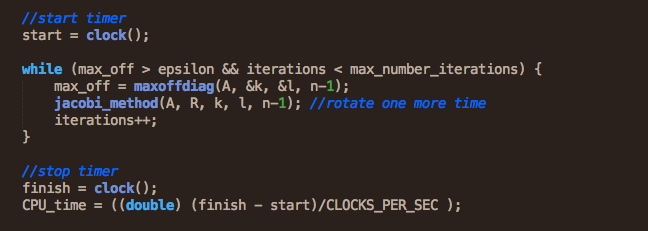
\includegraphics[width = 130mm]{jacobi_method.png}\\
  \caption{Figuren viser hovedtrekkene i hvordan Jacobis metode kan implementeres i C++, og hvordan CPU-tiden til denne prosessen kan beregnes.}\label{fig:jacobi}
  \end{center}
\end{figure}
\FloatBarrier

\subsubsection{To elektroner som vekselvirker}
Jacobis metode kan også brukes i det tilfellet hvor to elektroner vekselvirker med hverandre via Coulombkrefter. Vi skal se på hva som skjer når vi har $\omega_r$ = 0.01, $\omega_r$ = 0.5, $\omega_r$ = 1 og $\omega_r$ = 5, når vi befinner oss i grunntilstanden med $l$ = 0. Vi skal her se bort fra massesenter-energien $E_R$. Fremgangsmåten for dette oppsettet er tilnærmet likt som i forrige seksjon, så lenge vi husker å endre potensialet fra $\rho$ til $\omega_r^2\rho^2 + 1/\rho $. Diagonalelementene i matrisen $A$ vil da være på formen $d_i = 2/h^2 + \omega_R^2\rho_i^2 + 1/\rho_i$. For de gitte oscillator-frekvensene vet vi at den analytiske løsningen er gitt ved 

HVA DASKJDFSKJFHKSDJF


\subsection{Bruk av Armadillo}
En annen metode å løse egenverdiproblemet på, er å ved hjelp av Armadillos innebygde funksjon \texttt{eig$\_$sym}. Denne funksjonen finner enkelt eigenverdiene og eigenvektorene vi er ute etter. Funksjonen \texttt{eig$\_$sym(eigenvalues, R, A)} tar inn matrisen $A$ og finner dens eigenverdier og eigenvektorer. Eigenverdiene lagres i vektoren \textit{eigenvalues}, mens eigenvektorene lagres som kolonner i matrisen $R$. Siden vi nå har to ulike løsningsmetoder, kan vi enkelt sammenligne resultatene for å se om de stemmer overens med hverandre.



\section{Resultater}
Tabell \ref{tab:jacobi} og \ref{tab:armadillo} viser resultatene fra Jacobis metode og Armadillo-metoden for ulike verdier av $n$ i tilfellet hvor vi ikke hadde noen vekselvirkning. Her er $\rho_{max}$ = 5.0.

\FloatBarrier
\begin{table}[!ht]
\centering
\caption{De tre minste eigenverdiene for ulike verdier av $n$, sammen med beregningstiden og antall iterasjoner. Resultatene fra armadillo-metoden er tatt med for sammenligning.}
\label{tab:jacobi}
\begin{tabular}{|c|c|c|c|c|c|}
\hline
$\textbf{n}$      &  $\textbf{Eigenverdier}_{Jacobi}$ & $\textbf{CPU [s]}$ & $\textbf{Iterasjoner}$ \\ 
\hline
$10$     & (2.919484, 6.583038, 9.936657) &  0.00022600 & 105               \\ 
\hline
$50$ & (2.996871, 6.984342, 10.96193)     & 0.091970     & 3 852             \\ 
\hline
$100$ & (2.999219, 6.996094, 10.99066)     & 1.0987      & 16 217         \\ 
\hline
$200$ & (2.999805, 6.999026, 10.99781)     & 17.236     & 66 065             \\ 
\hline
$300$ & (2.999913, 6.999568, 10.99914)     & 90.121    & 149 879               \\ 
\hline
$310$ & (2.999919, 6.999596, 10.99921)     &  118.81   & 160 171     \\ 
\hline       
\end{tabular}
\end{table}
\FloatBarrier

\FloatBarrier
\begin{table}[!ht]
\centering
\caption{Tabellen viser de tre laveste eigenverdiene samt beregningstiden ved bruk av Armadillo-metoden.}
\label{tab:armadillo}
\begin{tabular}{|c|c|c|c|c|c|}
\hline
\textbf{n}     &  $\textbf{Eigenverdier}_{armadillo}$  &  $\textbf{CPU}_{armadillo} [s]$  \\ 
\hline
10     & (2.919484,   6.583038,   9.936657)  &8.0000E-05     \\ 
\hline
50 & (2.996871, 6.984342, 10.96193)  &     0.00062900        \\ 
\hline
100 & (2.999219, 6.996094, 10.99066)  & 0.0034070         \\ 
\hline
200 & (2.999805, 6.999026, 10.99781)  & 0.013732     \\ 
\hline   
300 & (2.999913, 6.999568, 10.99914) & 0.032447      \\ 
\hline   
310 & (2.999919, 6.999596, 10.99921)  & 0.035778     \\ 
\hline   
\end{tabular}
\end{table}
\FloatBarrier


I tabell \ref{tab:jacobi_interact} vises resultatene for tilfellet \textbf{med} vekselvirkning. Her er $n$ = 200 og $\rho_{max}$ = 5 konstant, mens verdien til $\omega_R$ varierer. 

\FloatBarrier
\begin{table}[!ht]
\centering
\caption{I tabellen vises de numerisk beregnede eigenverdiene til grunntilstanden for ulike verdier av oscillatorrekvensen $\omega_R$, sammen med den tilnærmede og eksakte løsningen.}
\label{tab:jacobi_interact}
\begin{tabular}{|c|c|c|c|c|c|}
\hline
$\omega_R$  &  $\textbf{Eigenverdi (numerisk)}$   \\ 
\hline
0.01     & 0.8407035     \\ 
\hline
0.5 & 2.230821           \\ 
\hline
1 & 4.057058       \\ 
\hline
5 & 17.42822    \\ 
\hline   
\end{tabular}
\end{table}
\FloatBarrier

\section{Diskusjon}
2b)

Vi ser av tabell \ref{tab:jacobi} at vi trengte $n \approx$ 200 grid-points for å få de tre laveste eigenverdiene med fire gjeldende siffere etter desimalen. Vi satte da $\rho_{max} = 5.0$.\\

Antallet iterasjoner, eller rotasjoner, som trengtes før alle ikke-diagonal elementene ble tilnærmet lik null varierte med antall grid-points $n$. I tilfellet hvor $n = 200$ trengte vi 66 065 iterasjoner. Vi kan finne en funksjon som forteller oss om antall iterasjoner som funksjon av størrelsen på matrisen. En liten regresjonsanalyse av resultatene i tabell \ref{tab:jacobi} gir oss noe à la
\[ iterasjoner = 1.69n^2 - 7.9n + 29.8 \] 

aser at vi får de samme egenverdiene, noe som er betryggende. MEN betraktelig forskjell i beregningstid. arma

The convergence rate of the Jacobi method is however poor, one needs typically 3n2 - 5n2 ro- tations and each rotation requires 4n operations, resulting in a total of 12n3 - 20n3 operations in order to zero out non-diagonal matrix elements. Although the classical Jacobi algorithm performs badly compared with methods based on tridiagonalization, it is easy to parallelize.
The slow convergence is related to the fact that when a new rotation is performed, matrix elements which were previously zero, may change to non-zero values in the next rotation.

 "Comment your results (here you could for example compute the time needed for both algorithms for a given dimensionality of the matrix)."
 jævlig treig
 
 2c) unit test: bra
 
 2d) Kommenter resultatene for den laveste egenverdien (tilstanden) som funksjon av ulike omega. Hva er trenden? tilstanden øker jo større omega (oscillatorfrekvens). Hvorfor? 
 Sammenlign med resultatene fra artikkelen...
 

\section{Konklusjon}
fgddfg


\section{Vedlegg}
Alle koder og resultater som er brukt i rapporten finnes på Github-adressen: https://github.com/livewj/Project-1



\bibliography{Referanser}
\begin{thebibliography}{9}

\bibitem{squires}
  Kursets offisielle Github-side $\textit{FYS3150 - Computational Physics}$
  https://github.com/CompPhysics/ComputationalPhysics,
  03.09.2016  
  
\bibitem{}
  Slides fra kursets offisielle nettside
  "Matrices and linear algebra":
   http://compphysics.github.io/ComputationalPhysics/doc/web/course, 24.09.16
  "How to write a scientific project, with examples":
  http://compphysics.github.io/ComputationalPhysics/doc/pub/projectwriting/html/projectwriting.html, 24.09.17
   
\bibitem{}
   M. Hjort-Jensen: Computational physics, lecture notes 2015. Fysisk institutt, UiO, 2016.

   
\end{thebibliography}

\end{document}